\documentclass[12pt,a4paper]{article}
\usepackage[utf8]{inputenc}
\usepackage[spanish]{babel}
\usepackage{amsmath}
\usepackage{amsfonts}
\usepackage{amssymb}
\usepackage{makeidx}
\usepackage{graphicx}
\usepackage[left=2cm,right=2cm,top=2cm,bottom=2cm]{geometry}

\author{Felipe Alvarado Galicia}
\title{CINEMÁTICA DIRECTA E INVERSA DE MANIPULADORES PARALELOS}
\date{Profesor:Carlos Enrique Moran Garabito\\
Materia: Cinematica de Robots\\
29 de octubre de 2019}

\begin{document}
\maketitle
 
\includegraphics[scale=1]{logo1.png}\\
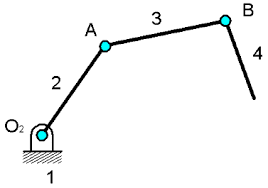
\includegraphics[scale=1]{imag5.png} 
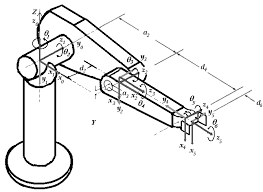
\includegraphics[scale=1]{imag8.png}\\\\\\\\\\\\\\\\\\\\\\\\\\\\\\\\\\\\\\\\\\\\\\

\tableofcontents

\section{Cinematica directa de manipuladores paralelos}
En la cinemática directa de robots paralelos el problema es determinar la posición del efector final en función de las juntas activas. En general, la solución a este problema no es única, de ahí que la cinemática ha sido objeto de una intensa investigación, por ejemplo, el trabajo reportado por Merlet. Raghavan muestra la solución de la cinemática directa de un manipulador paralelo resolviendo en función de un polinomio. Merlet, Tsai y Ángeles mostraron, de igual manera, que el problema de la cinemática directa es reducir las ecuaciones de posición a un polinomio en función de las variables activas. Sin embargo, la solución del polinomio no asegura la correcta evolución de las variables de las juntas activas y no considera a las juntas pasivas, al ejecutar una tarea dada. Por otro lado, no hay algoritmo conocido que permita la fácil determinación de una postura única para la plataforma móvil.\\\\
Es importante hacer hincapié en el problema del resultado de la cinemática directa por polinomio. El cálculo puede implicar un gran número de operaciones y por lo tanto puede ser muy sensible a errores numéricos de redondeo; por esta razón la comprobación de la validez de las soluciones con la cinemática inversa es normalmente necesaria.\\\\
La solución de la cinemática directa e inversa, utilizando la integración de la cinemática diferencial, es particularmente importante para los manipuladores de cadenas cinemáticas cerradas cuyas soluciones no existen, son difíciles de obtener, o son demasiado complejas para ser tratadas; el trabajo de Campos, A., R. Guenther, and D. Martins, sobre robots redundantes o paralelos, constituye un buen ejemplo de esto.

\section{Cinematica inversa de manipuladores paralelos}
En robots paralelos, la cinemática inversa consiste en encontrarlas variables de las juntas activas y pasivas en función de las coordenadas del efector final del robot y puede ser utilizada para controlarla posición del efector final. El modelo cinemático de este tipo de robots tiene ecuaciones algebraicas con múltiples soluciones.\\\\
La solución de la cinemática directa e inversa, utilizando la integración de la cinemática diferencial, es particularmente importante para los manipuladores de cadenas cinemáticas cerradas cuyas soluciones no existen, son difíciles de obtener, o son demasiado complejas para ser tratadas; el trabajo de Campos, A., R. Guenther, and D. Martins[12], sobre robots redundantes o paralelos, constituye un buen ejemplo de esto.\\

\section{Bibliografía}
http://www.scielo.org.mx/scielo.php





\end{document}